\documentclass{beamer}
\usepackage[utf8]{inputenc}
\usepackage{graphicx, epsfig}
\usepackage{amsmath,mathrsfs,amsfonts,amssymb}
%\usepackage{subfig}
\usepackage{floatflt}
\usepackage{epic,ecltree}
\usepackage{mathtext}
\usepackage{fancybox}
\usepackage{fancyhdr}
\usepackage{multirow}
\usepackage{enumerate}
\usepackage{epstopdf}
\usepackage{multicol}
\usepackage{algorithm}
\usepackage[noend]{algorithmic}
\def\algorithmicrequire{\textbf{Input:}}
\def\algorithmicensure{\textbf{Output:}}
\usetheme{default}%{Singapore}%{Warsaw}%{Warsaw}%{Darmstadt}
\usecolortheme{default}
\setbeamertemplate{footline}[page number]{}
\setbeamerfont{title}{size=\Huge}

\newcommand{\bt}{\mathbf{t}} 
\newcommand{\bu}{\mathbf{u}} 
\newcommand{\bv}{\mathbf{v}} 
\newcommand{\bw}{\mathbf{w}} 
\newcommand{\bx}{\mathbf{x}} 
\newcommand{\bz}{\mathbf{z}} 
\newcommand{\by}{\mathbf{y}} 

\newcommand{\bI}{\mathbf{I}} 
\newcommand{\bT}{\mathbf{T}} 
\newcommand{\bX}{\mathbf{X}} 
\newcommand{\bZ}{\mathbf{Z}} 

\newcommand{\bepsilon}{\boldsymbol{\epsilon}}
\newcommand{\bmu}{\boldsymbol{\mu}}
\newcommand{\blambda}{\boldsymbol{\lambda}}
\newcommand{\bsigma}{\boldsymbol{\sigma}}
\newcommand{\bSigma}{\boldsymbol{\Sigma}}

\newcommand{\bbE}{\mathbb{E}} 
\newcommand{\bbP}{\mathbb{P}} 
\newcommand{\bbR}{\mathbb{R}} 

\newcommand{\cL}{\mathcal{L}} 
\newcommand{\cN}{\mathcal{N}} 
\newcommand{\cS}{\mathcal{S}} 
\newcommand{\cX}{\mathcal{X}} 

\newcommand{\btheta}{\boldsymbol{\theta}} 
\newcommand{\bphi}{\boldsymbol{\phi}} 

\DeclareMathOperator*{\argmin}{arg\,min}
\DeclareMathOperator*{\argmax}{arg\,max}

%\definecolor{beamer@blendedblue}{RGB}{15,120,80}
%----------------------------------------------------------------------------------------------------------
\title[\hbox to 56mm{Deep Generative Models  \hfill\insertframenumber\,/\,\inserttotalframenumber}]
{Deep Generative Models \\ Lecture 8}
\author[Roman Isachenko]{\\Roman Isachenko}
\institute[MIPT]{Moscow Institute of Physics and Technology \\
}
\date{2020}
%--------------------------------------------------------------------------------
\begin{document}
%--------------------------------------------------------------------------------
\begin{frame}
%\thispagestyle{empty}
\titlepage
\end{frame}
%=======
\begin{frame}{Wasserstein GAN}
	\begin{block}{Wasserstein distance}
		\vspace{-0.4cm}
		\[
			W(\pi, p) = \inf_{\gamma \in \prod(\pi, p)} \bbE_{(\bx, \by) \sim \gamma} \| \bx - \by \| =  \inf_{\gamma \in \prod(\pi, p)} \int \| \bx - \by \| \gamma (\bx, \by) d \bx d \by
		\]
	\end{block}
	The infimum across all possible joint distributions in $\prod(\pi, p)$ is intractable.
	\begin{block}{Kantorovich-Rubinstein duality}
		\[
			W(\pi, p) = \frac{1}{K} \max_{\| f \|_L \leq K} \left[ \bbE_{\bx \sim \pi} f(\bx)  - \bbE_{\bx \sim p} f(\bx)\right],
		\]
		where $\| f \|_L \leq K$ are $K-$Lipschitz continuous functions ($f: \cX \rightarrow \bbR$)
		\[
			|f(\bx_1) - f(\bx_2)| \leq K \| \bx_1 - \bx_2 \|, \quad \text{for all } \bx_1, \bx_2 \in \cX.
		\]
	\end{block}
	\vfill
	\hrule\medskip 
	{\scriptsize \href{https://arxiv.org/abs/1701.07875}{https://arxiv.org/abs/1701.07875}}
\end{frame}
%=======
\begin{frame}{Wasserstein GAN}
		\begin{block}{Kantorovich-Rubinstein duality}
		\[
			W(\pi, p) = \frac{1}{K} \max_{\| f \|_L \leq K} \left[ \bbE_{\bx \sim \pi} f(\bx)  - \bbE_{\bx \sim p} f(\bx)\right],
		\]
	\end{block}
	\begin{itemize}
		\item Now we have to ensure that $f$ is $K$-Lipschitz continuous.
		\item Let make $f(\bx, \phi)$ parametrized by parameters $\bphi$.
		\item If parameters $\phi$ lies in a compact set $\boldsymbol{\Phi}$ then $f(\bx, \bphi)$ will be $K$-Lipschitz continuous function. 
		\item Let clamp the parameters to a fixed box $\boldsymbol{\Phi} \in [-0.01, 0.01]^d$ after each gradient update.
	\end{itemize}
	{\footnotesize
	\[
		 \max_{\bphi \in \boldsymbol{\Phi}} \left[ \bbE_{\bx \sim \pi} f(\bx, \bphi)  - \bbE_{\bx \sim p} f(\bx, \bphi )\right] \leq  \max_{\| f \|_L \leq K} \left[ \bbE_{\bx \sim \pi} f(\bx)  - \bbE_{\bx \sim p} f(\bx)\right] = K \cdot W(\pi || p)
	\]}
	\vfill
	\hrule\medskip 
	{\scriptsize \href{https://arxiv.org/abs/1701.07875}{https://arxiv.org/abs/1701.07875}}
\end{frame}
%=======
\begin{frame}{Wassestein GAN}
	\begin{block}{Vanilla GAN objective}
		\vspace{-0.3cm}
		\[
			\min_{G} \max_D \bbE_{\pi(\bx)} \log D(\bx) + \bbE_{p(\bz)} \log (1 - D(G(\bz)))
		\]
	\end{block}
	\begin{block}{WGAN objective}
		\vspace{-0.6cm}
		\[
		\min_{G} W(\pi, p) = \min_{G} \frac{1}{K} \max_{\bphi \in \boldsymbol{\Phi}} \left[ \bbE_{\bx \sim \pi} f(\bx, \bphi)  - \bbE_{\bz \sim p} f(G(\bz), \bphi )\right].
		\]
	\end{block}
	\begin{itemize}
		\item Discriminator $D$ is similar to the function $f$, but not the same (it is not a classifier anymore). In the WGAN model, function $f$ is usually called $\textit{critic}$.
		\item "Weight clipping is a clearly terrible way to enforce a Lipschitz constraint". If the clipping parameter is large, it is hard to train the critic till optimality. If the clipping parameter is too small, it could lead to vanishing gradients.
	\end{itemize}
	\vfill
	\hrule\medskip 
	{\scriptsize \href{https://arxiv.org/abs/1701.07875}{https://arxiv.org/abs/1701.07875}}
\end{frame}
%=======
\begin{frame}{Wasserstein GAN}
	\begin{figure}
		\centering
		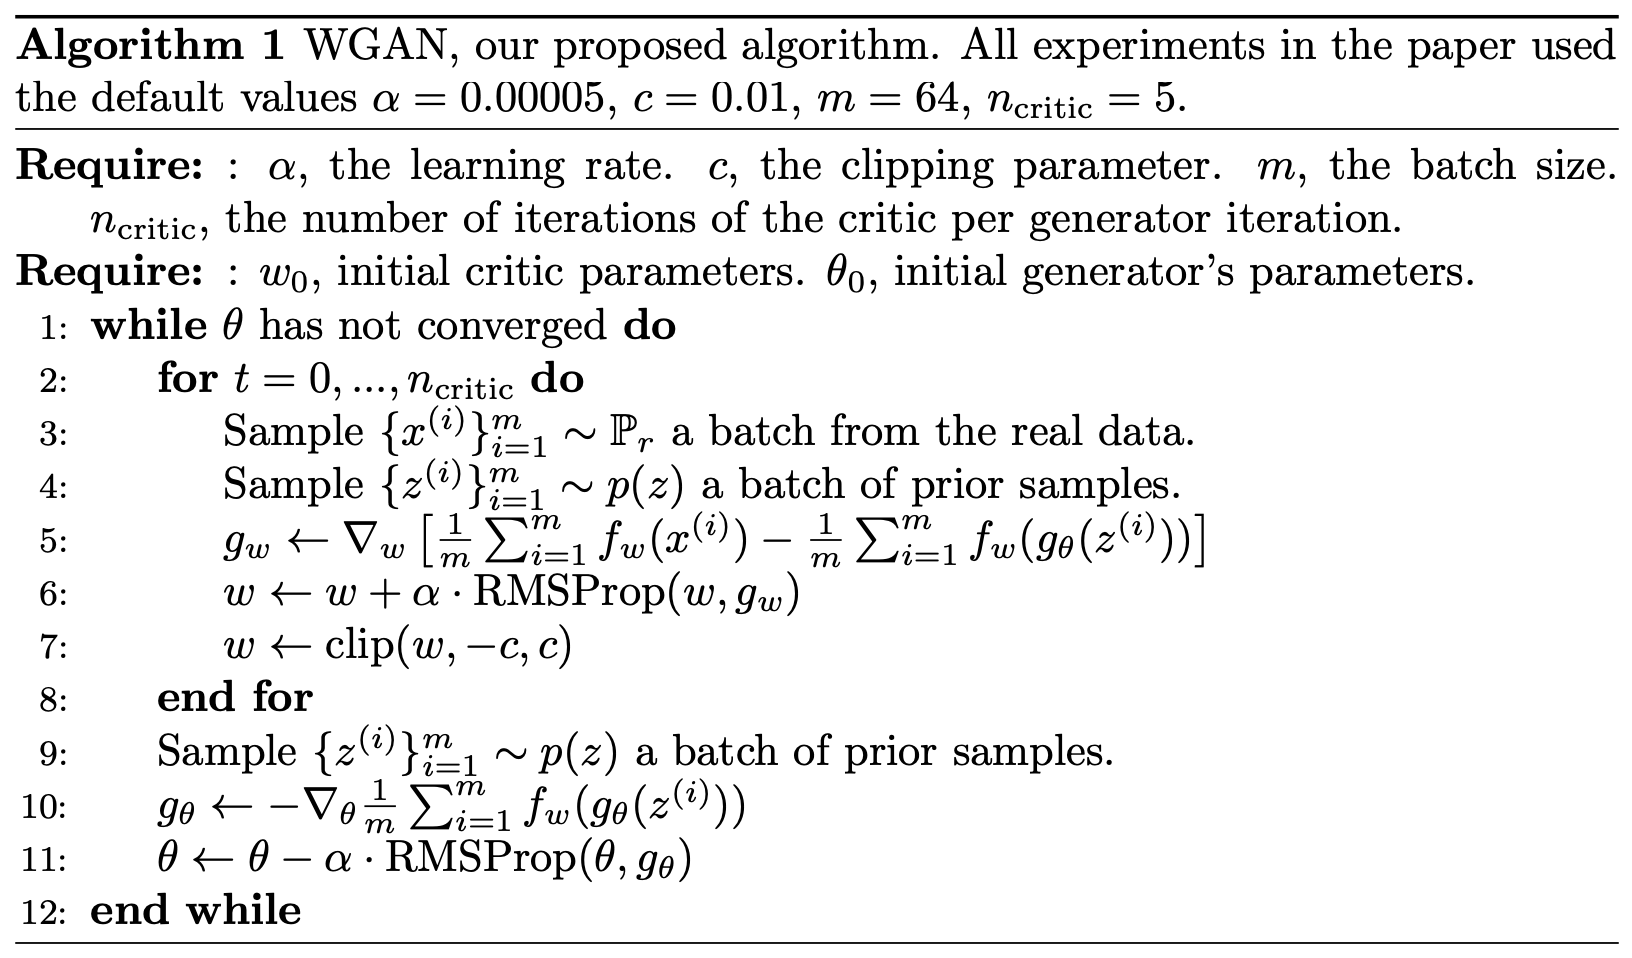
\includegraphics[width=1.0\linewidth]{figs/wgan_pseudocode}
	\end{figure}
	\vfill
	\hrule\medskip 
	{\scriptsize \href{https://arxiv.org/abs/1701.07875}{https://arxiv.org/abs/1701.07875}}
\end{frame}
%=======
\begin{frame}{Wasserstein GAN}
	\begin{figure}
		\centering
		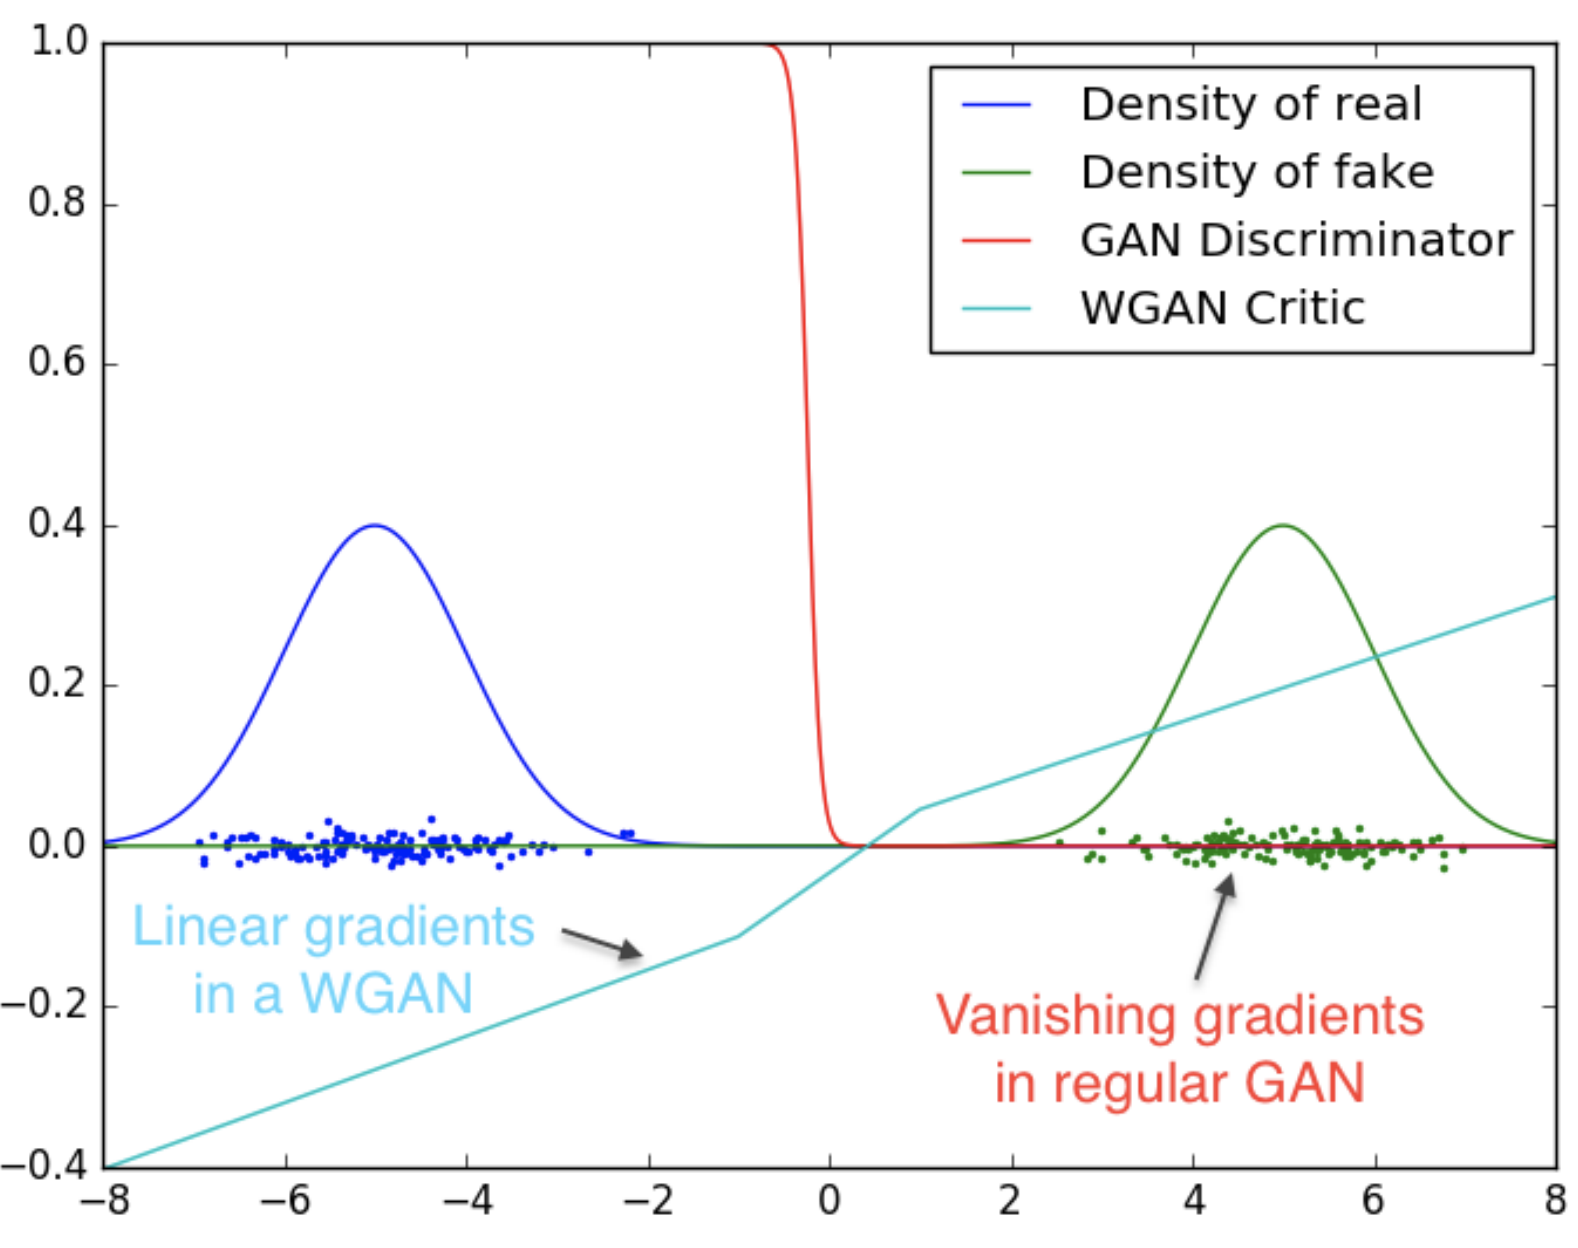
\includegraphics[width=0.8\linewidth]{figs/wgan_toy}
	\end{figure}
	\vfill
	\hrule\medskip 
	{\scriptsize \href{https://arxiv.org/abs/1701.07875}{https://arxiv.org/abs/1701.07875}}
\end{frame}
%=======
\begin{frame}{Wasserstein GAN}
	\begin{minipage}[t]{0.49\columnwidth}
		\begin{figure}
			\centering
			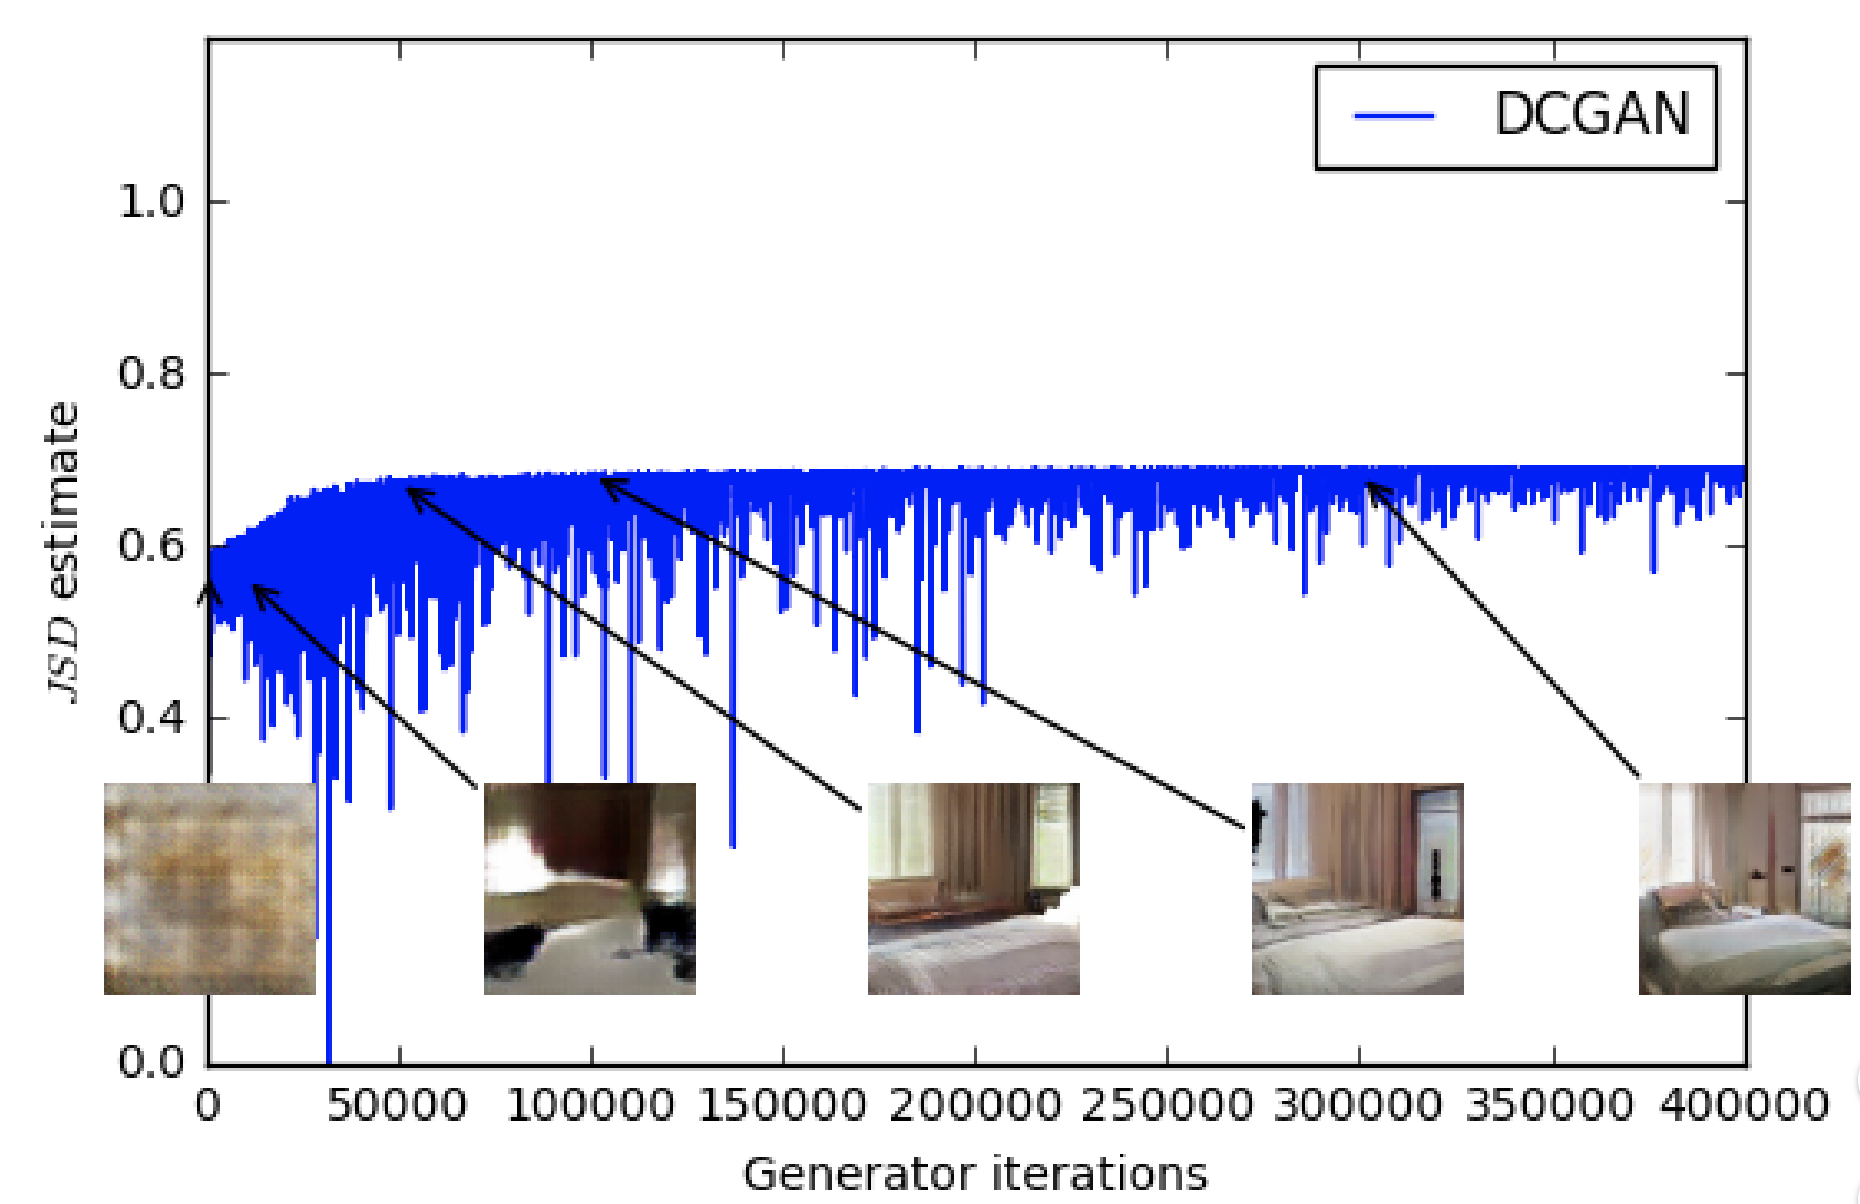
\includegraphics[width=1.0\linewidth]{figs/dcgan_quality}
		\end{figure}
	\end{minipage}%
	\begin{minipage}[t]{0.49\columnwidth}
		\begin{figure}
			\centering
			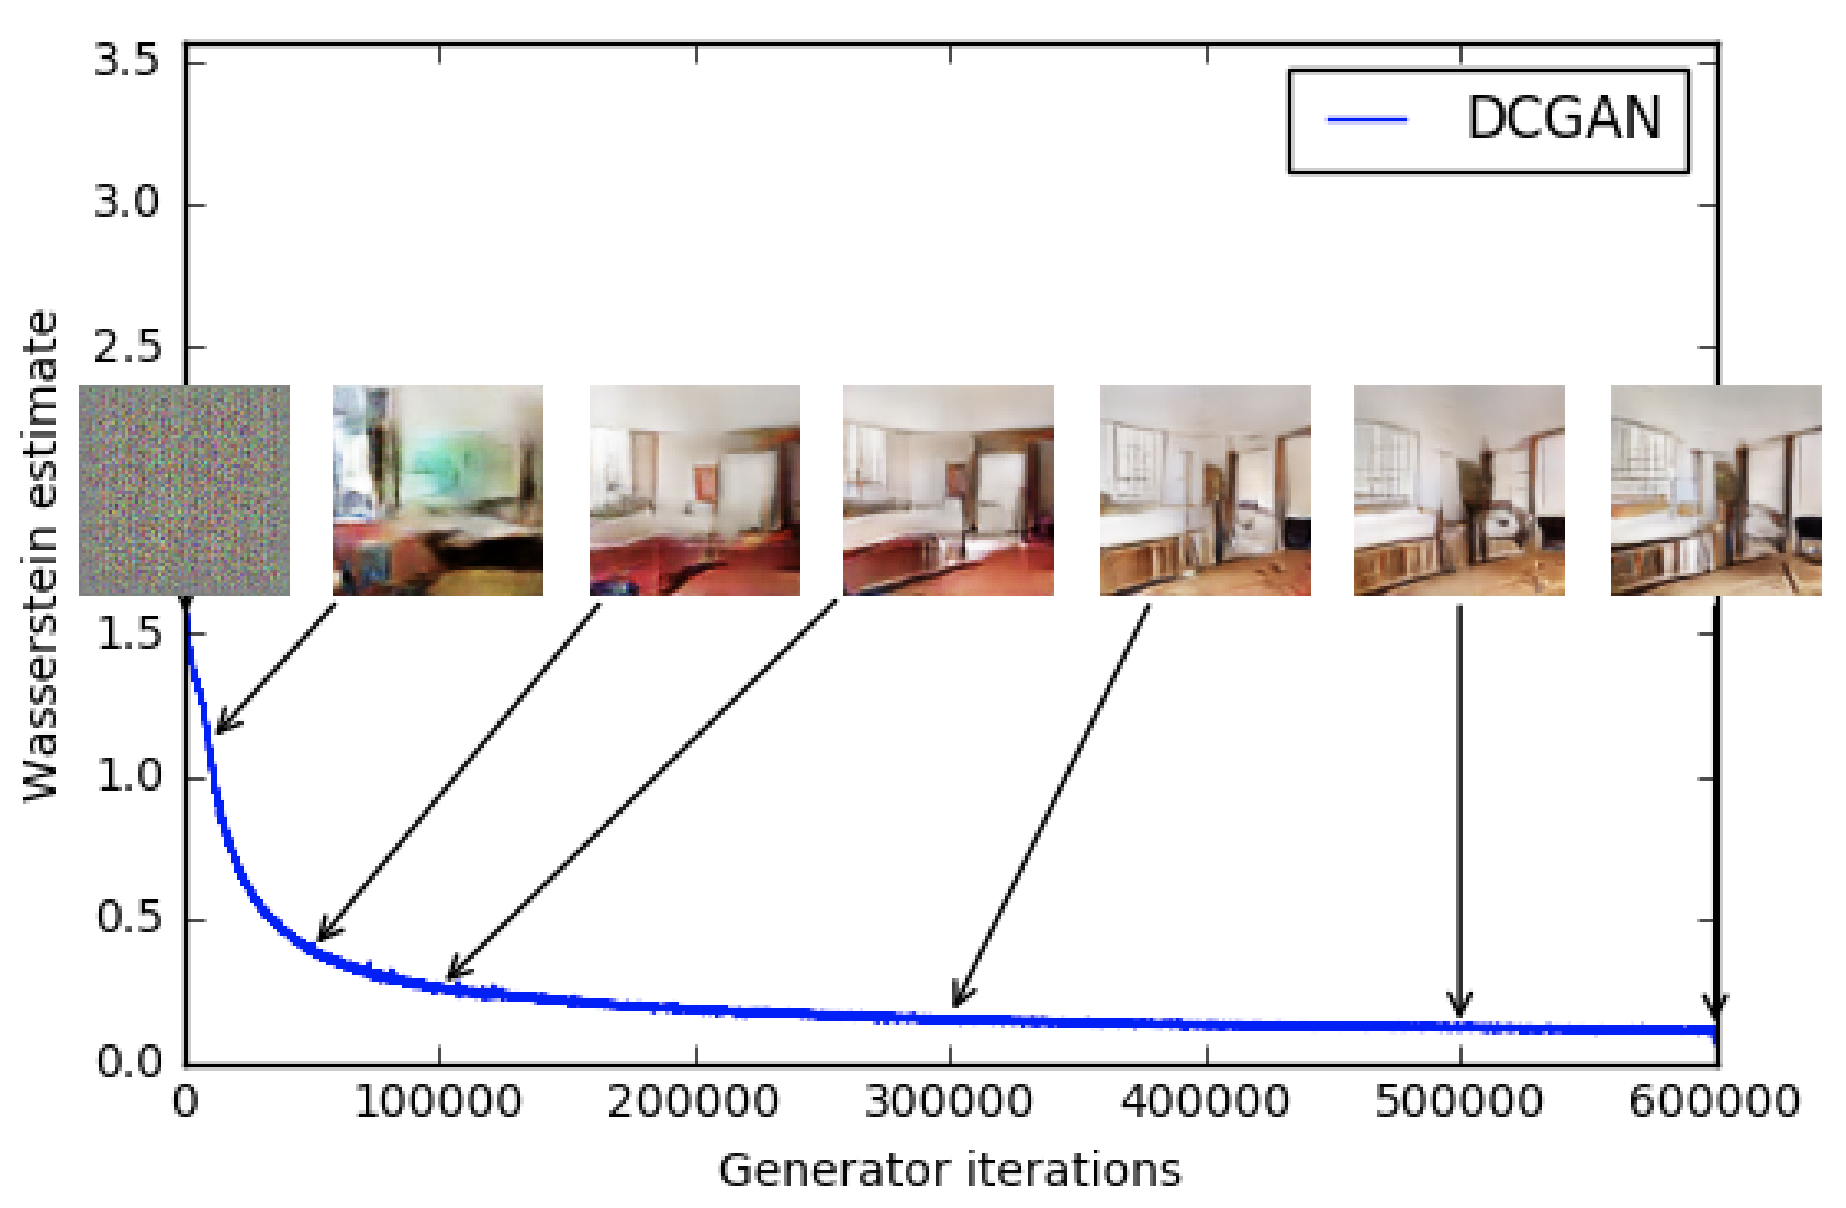
\includegraphics[width=1.0\linewidth]{figs/wgan_quality}
		\end{figure}
	\end{minipage}
	\begin{itemize}
		\item $JSD$ correlates poorly with the sample quality. Stays contast nearly maximum value $\log 2 \approx 0.69$.
		\item $W$ is highly correlated with the sample quality. 
	\end{itemize}
	\vfill
	\hrule\medskip 
	{\scriptsize \href{https://arxiv.org/abs/1701.07875}{https://arxiv.org/abs/1701.07875}}
\end{frame}
%=======
\begin{frame}{Wasserstein GAN}
	\begin{block}{WGAN converged without batch norm and constant number of filters}
		\begin{figure}
			\centering
			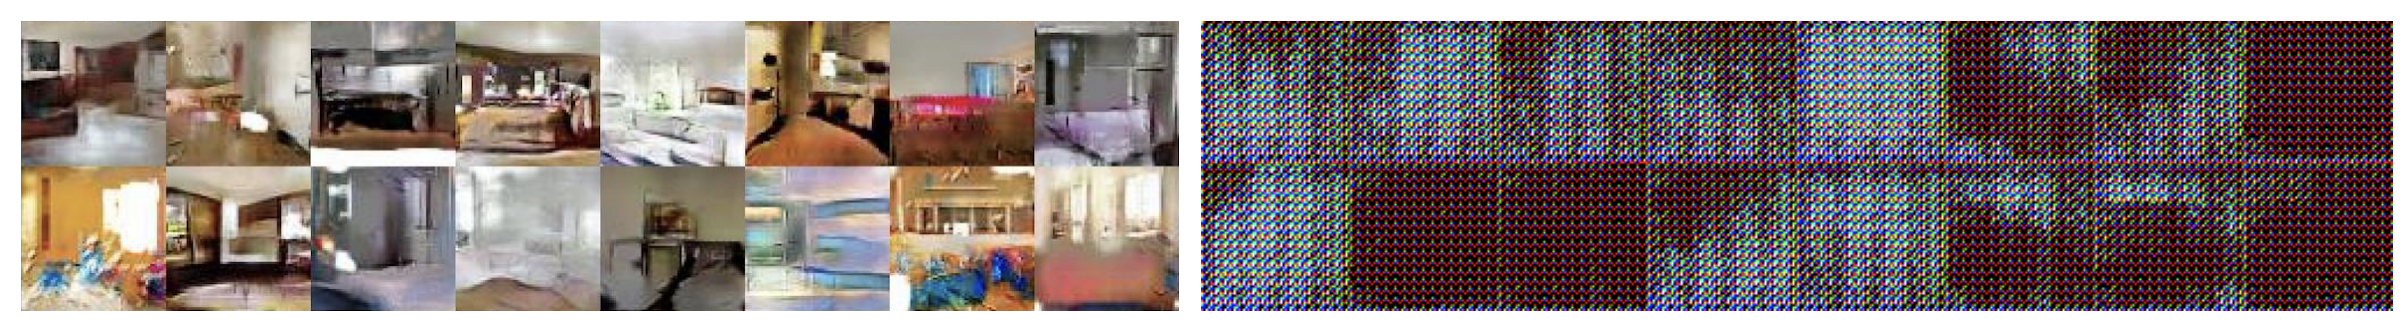
\includegraphics[width=1.0\linewidth]{figs/wgan_convergence}
		\end{figure}
	\end{block}
	\begin{block}{"In no experiment did we see evidence of mode collapse for the WGAN algorithm."}
		\begin{figure}
			\centering
			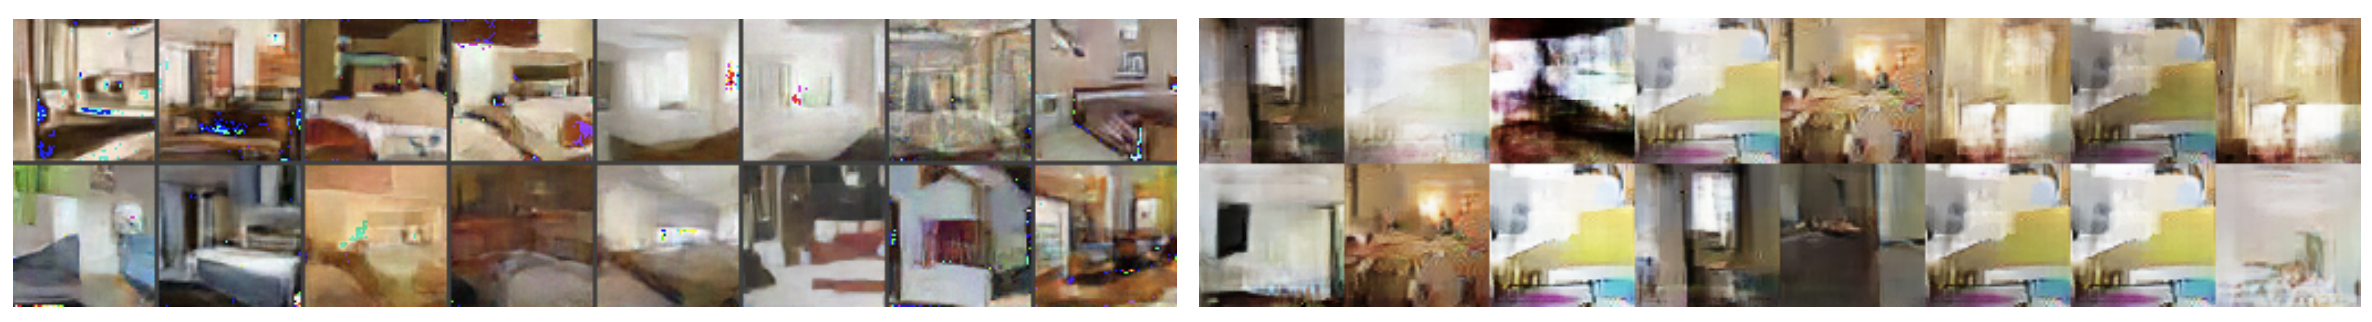
\includegraphics[width=1.0\linewidth]{figs/wgan_mode_collapse}
		\end{figure}
	\end{block}
	\vfill
	\hrule\medskip 
	{\scriptsize \href{https://arxiv.org/abs/1701.07875}{https://arxiv.org/abs/1701.07875}}
\end{frame}
%=======
\begin{frame}{Wasserstein GAN with Gradient Penalty}
	
	\begin{minipage}[t]{0.45\columnwidth}
		\vspace{0.2cm}
		The generator distribution is fixed and equals to the real distribution + Gaussian noise. \\
		Problems with weight clipping:
		\begin{itemize}
			\item The critic ignores higher moments of the data distribution.
			\item The gradient either grow or decay exponentially.
		\end{itemize}
	Gradient penalty makes the gradients  more stable.
	\end{minipage}%
	\begin{minipage}[t]{0.52\columnwidth}
		\begin{figure}
			\centering
			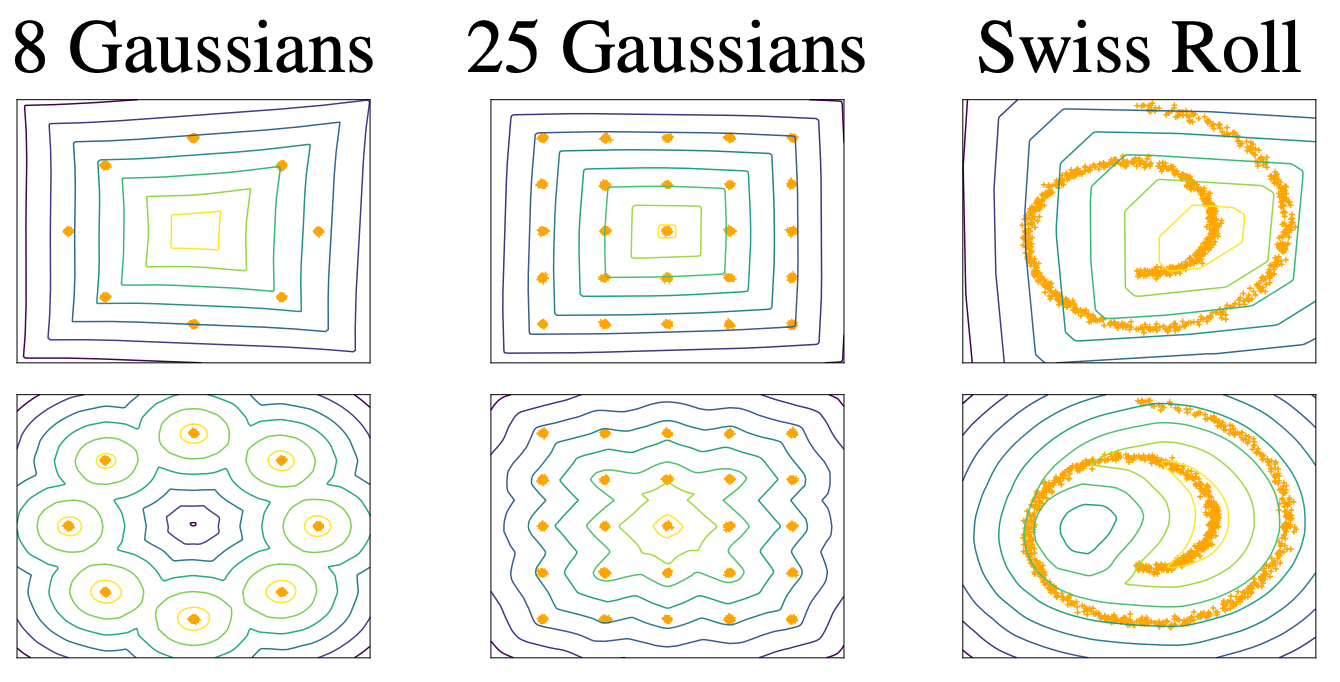
\includegraphics[width=0.95\linewidth]{figs/wgan_gp_toy}
		\end{figure}
		\begin{figure}
			\centering
			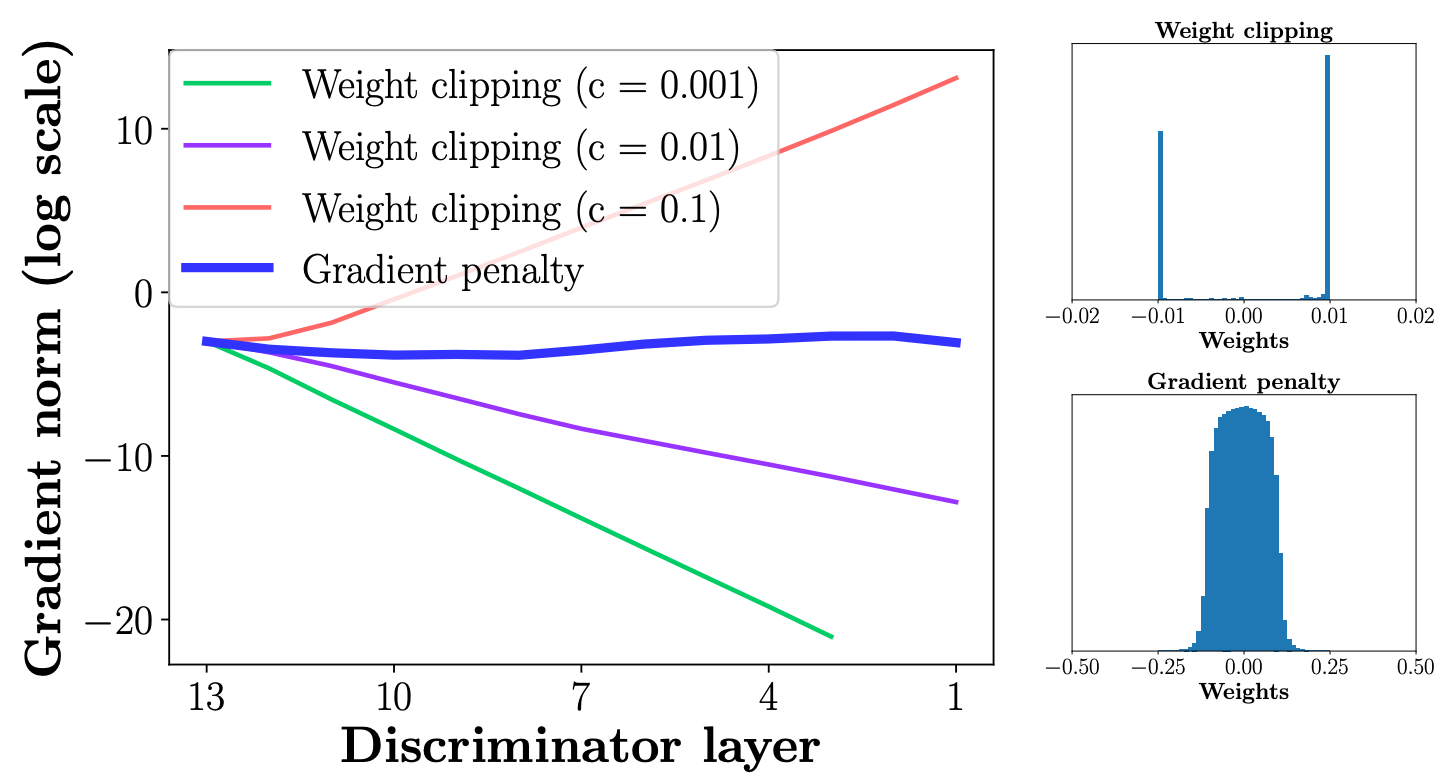
\includegraphics[width=0.95\linewidth]{figs/wgan_gp_weights}
		\end{figure}
	\end{minipage}
	
	\vfill
	\hrule\medskip 
	{\scriptsize \href{https://arxiv.org/abs/1704.00028}{https://arxiv.org/abs/1704.00028}}
	
\end{frame}
%=======
\begin{frame}{Wasserstein GAN with Gradient Penalty}
	\begin{block}{Theorem}
		Let $\pi(\bx)$ and $p(\bx)$ be two distribution in $\cX$, a compact metric space. Then, there is 1-Lipschitz function $f^*$ which is the optimal solution of 
		\[
			\max_{\| f \|_L \leq 1} \left[ \bbE_{\bx \sim \pi} f(\bx)  - \bbE_{\bx \sim p} f(\bx)\right].
		\]
		Let $\gamma$ be the optimal transportation plan between $\pi(\bx)$ and $p(\bx)$. Then, if $f^*$ is differentiable $\gamma(x = y) = 0$ and $\bx_t = t \bx + (1 - t) \by$ with $t \in [0, 1]$ it holds that
		\[
			\bbP_{(\bx, \by) \sim \gamma} \left[ \nabla f^*(\bx_t) = \frac{\by - \bx_t}{\| \by - \bx_t \|} = 1 \right].
		\]
	\end{block}
	\begin{block}{Corollary}
		$f^*$ has gradient norm 1 almost everywhere under $\pi(\bx)$ and $p(\bx)$.
	\end{block}
	\vfill
	\hrule\medskip 
	{\scriptsize \href{https://arxiv.org/abs/1704.00028}{https://arxiv.org/abs/1704.00028}}
\end{frame}
%=======
\begin{frame}{Wasserstein GAN with Gradient Penalty}
	A differentiable function is 1-Lipschtiz if and only if it has gradients with norm at most 1 everywhere.
	\begin{block}{Gradient penalty}
		\[
			W(\pi, p) = \underbrace{\bbE_{\bx \sim \pi} f(\bx)  - \bbE_{\bx \sim p} f(\bx)}_{\text{original critic loss}} + \lambda \underbrace{\bbE_{\hat{\bx}} \left[ \left( \| \nabla_{\hat{\bx}} f(\hat{\bx}) \|_2 - 1 \right) ^ 2\right]}_{\text{gradient penalty}},
		\]
	\end{block}
	\begin{itemize}
		\item Samples $\hat{\bx}$ are uniformly sampled along straight lines between pairs of points from the data distribution $\pi(\bx)$ and the generator distribuiton $p(\bx | \btheta)$.
		\item Enforcing the unit gradient norm constraint everywhere is intractable, it turns out sifficient to enforce it only along these straight lines.
	\end{itemize}
	\vfill
	\hrule\medskip 
	{\scriptsize \href{https://arxiv.org/abs/1704.00028}{https://arxiv.org/abs/1704.00028}}
\end{frame}
%=======
\begin{frame}{Wasserstein GAN with Gradient Penalty}
	
	\begin{figure}
		\centering
		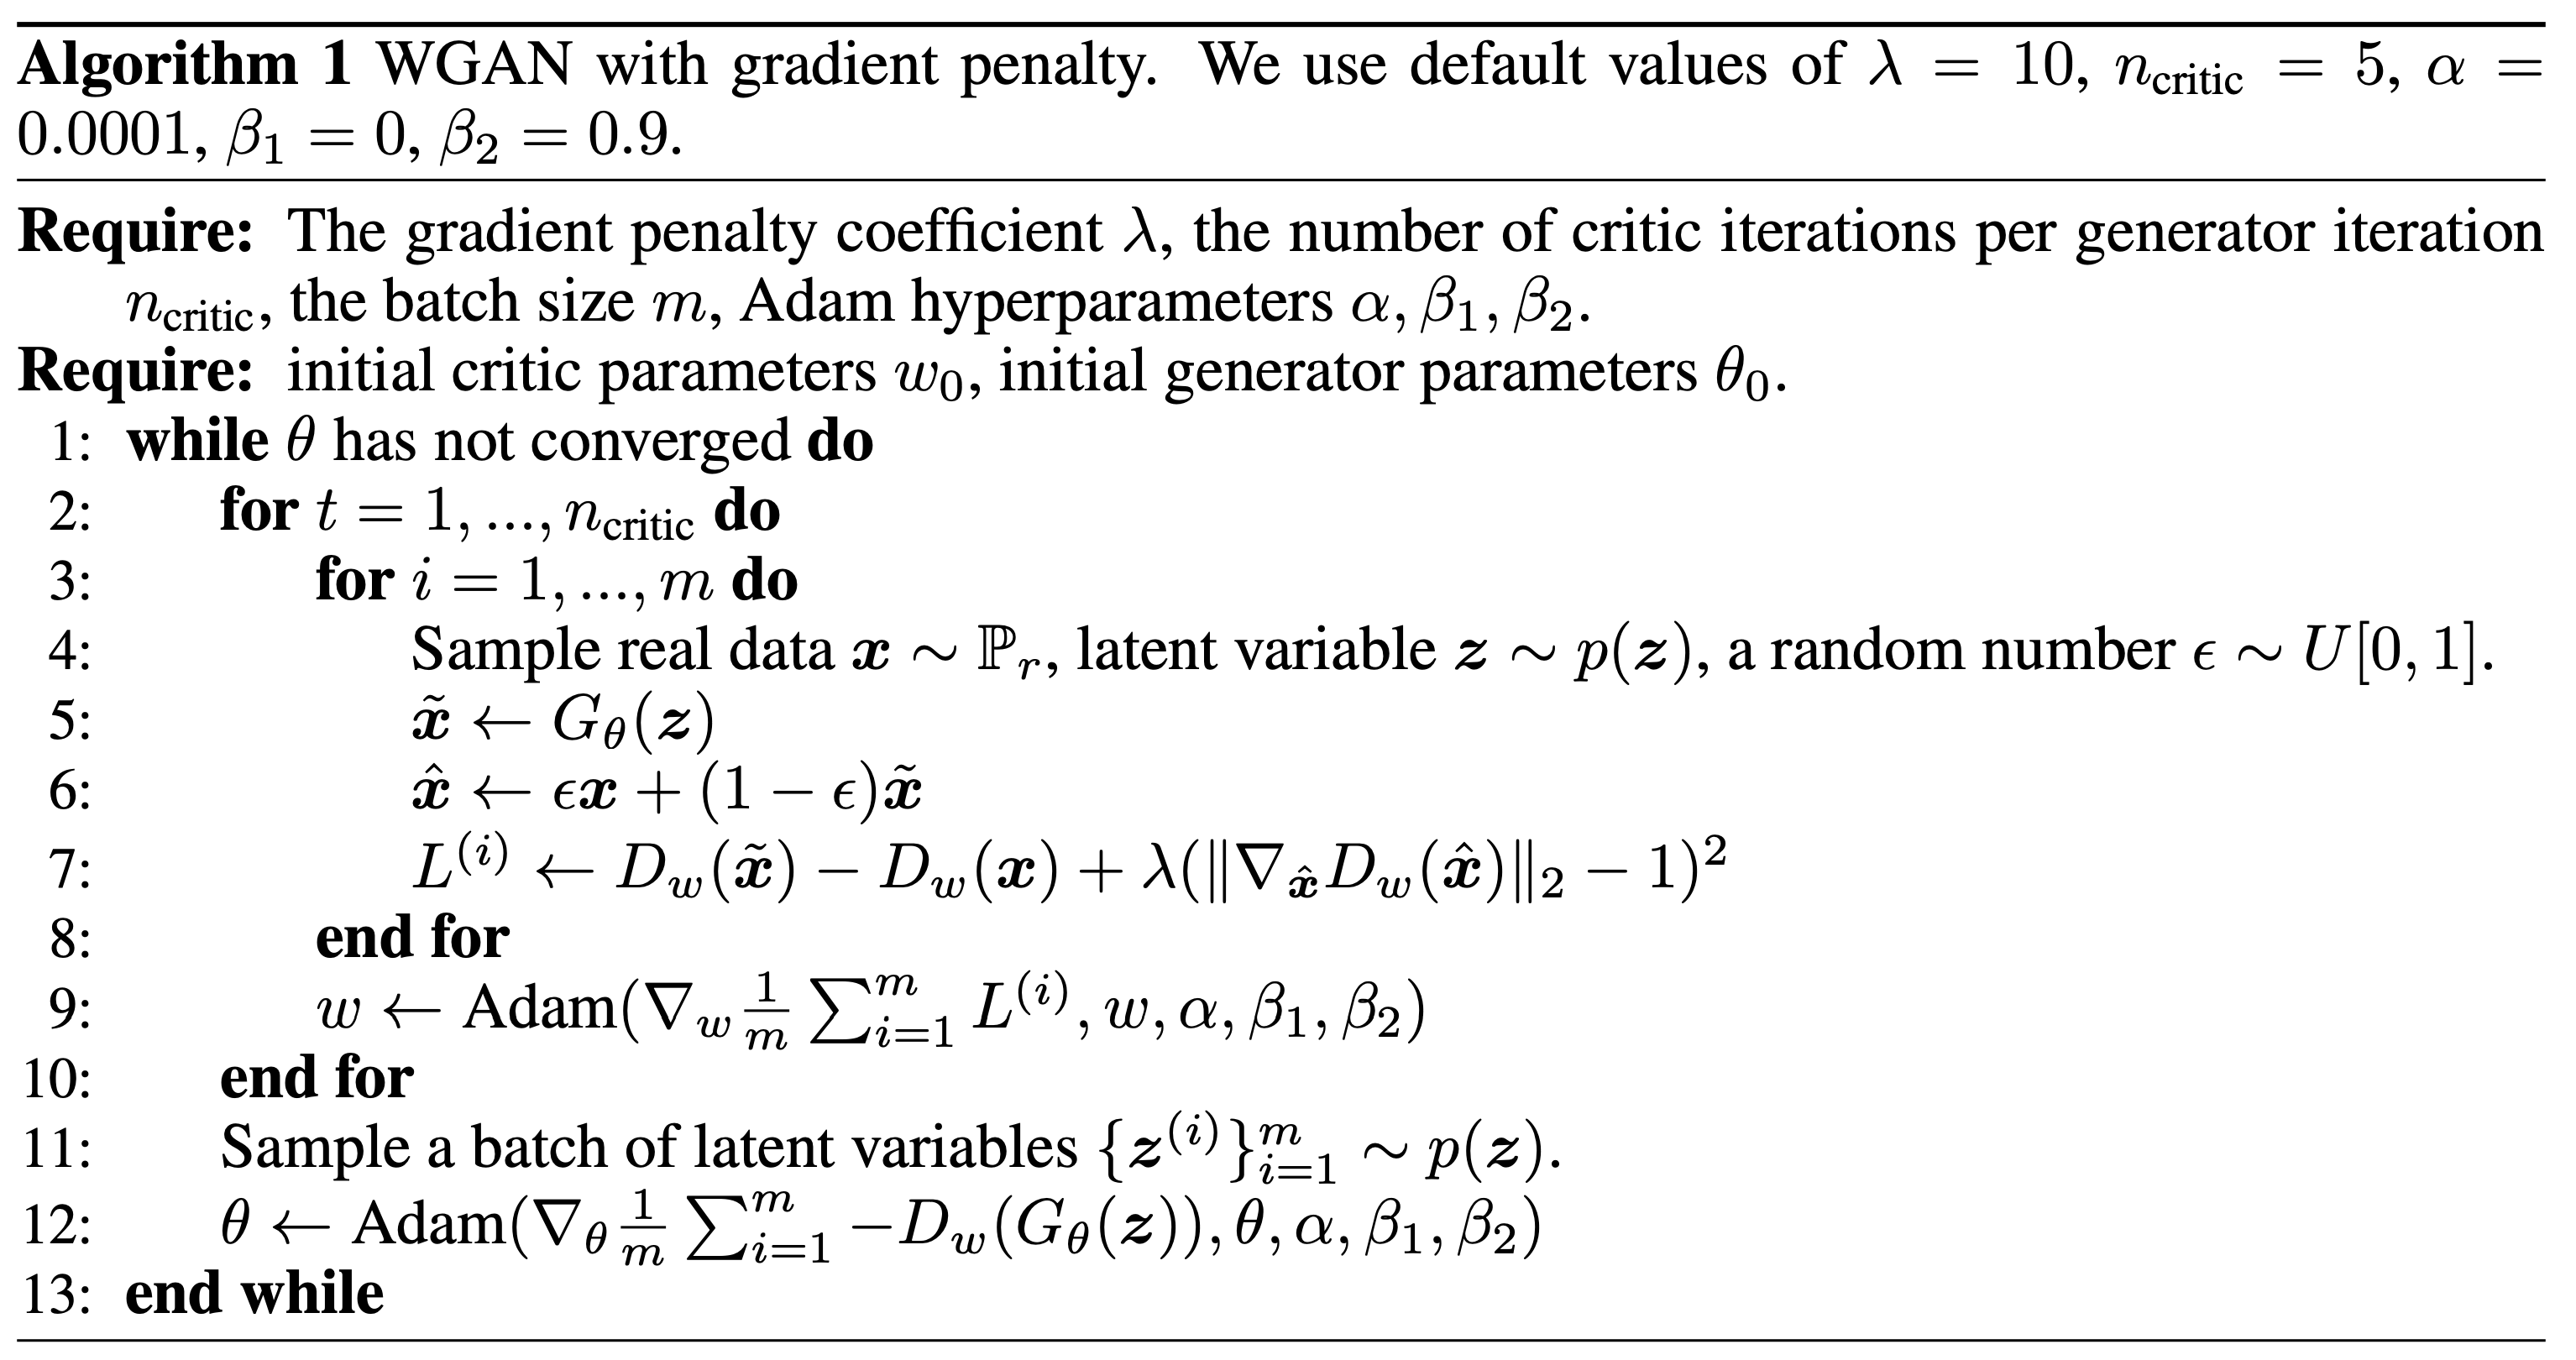
\includegraphics[width=1.0\linewidth]{figs/wgan_gp_pseudocode}
	\end{figure}
	
	\vfill
	\hrule\medskip 
	{\scriptsize \href{https://arxiv.org/abs/1704.00028}{https://arxiv.org/abs/1704.00028}}
	
\end{frame}
%=======
\begin{frame}{Wasserstein GAN with Gradient Penalty}
	\begin{figure}
		\centering
		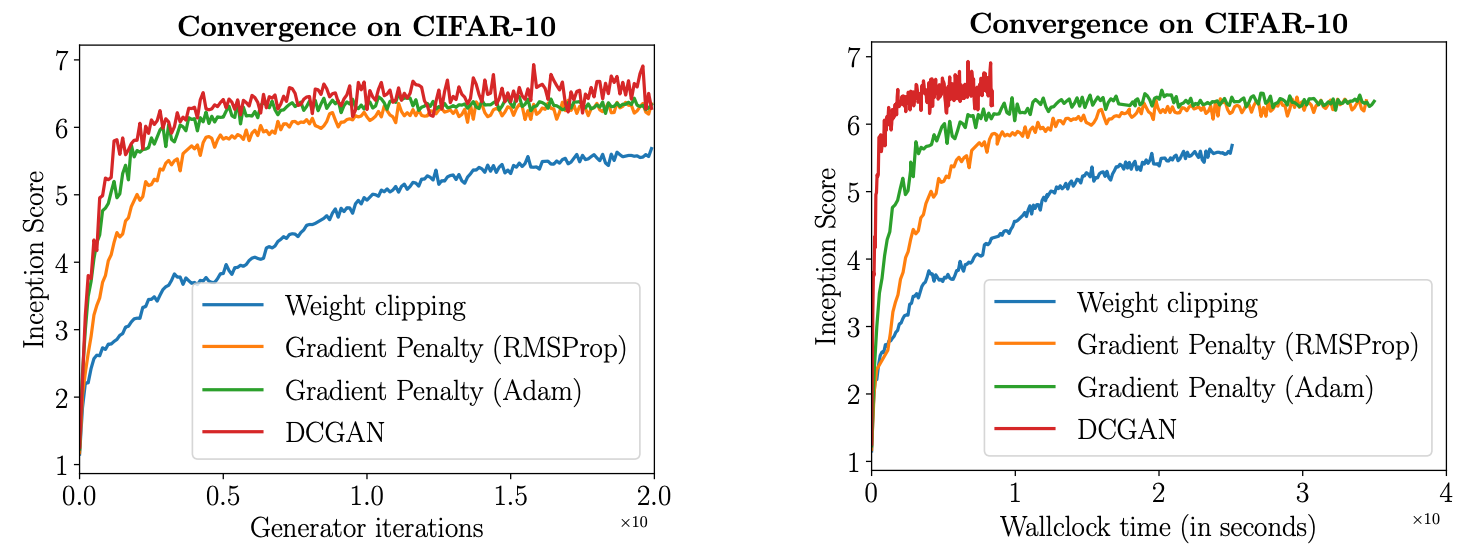
\includegraphics[width=0.9\linewidth]{figs/wgan_gp_convergence}
	\end{figure}
	\begin{figure}
		\centering
		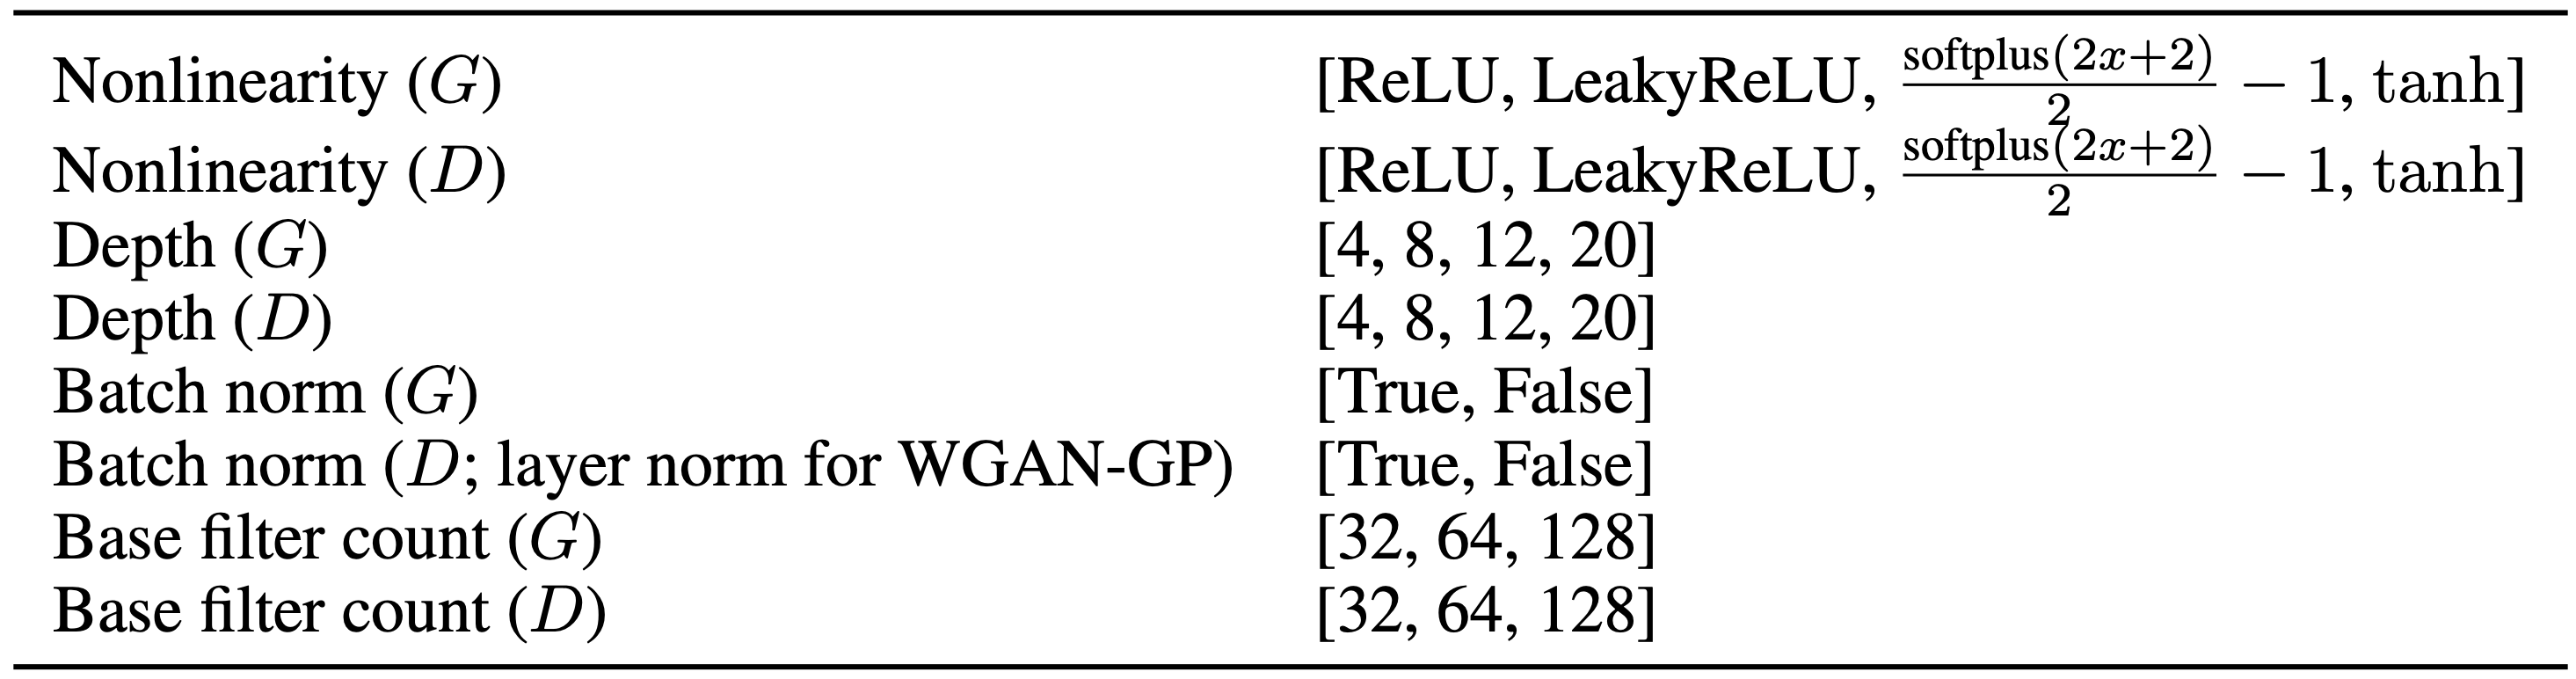
\includegraphics[width=0.65\linewidth]{figs/wgan_gp_model_space}
	\end{figure}
	\begin{figure}
		\centering
		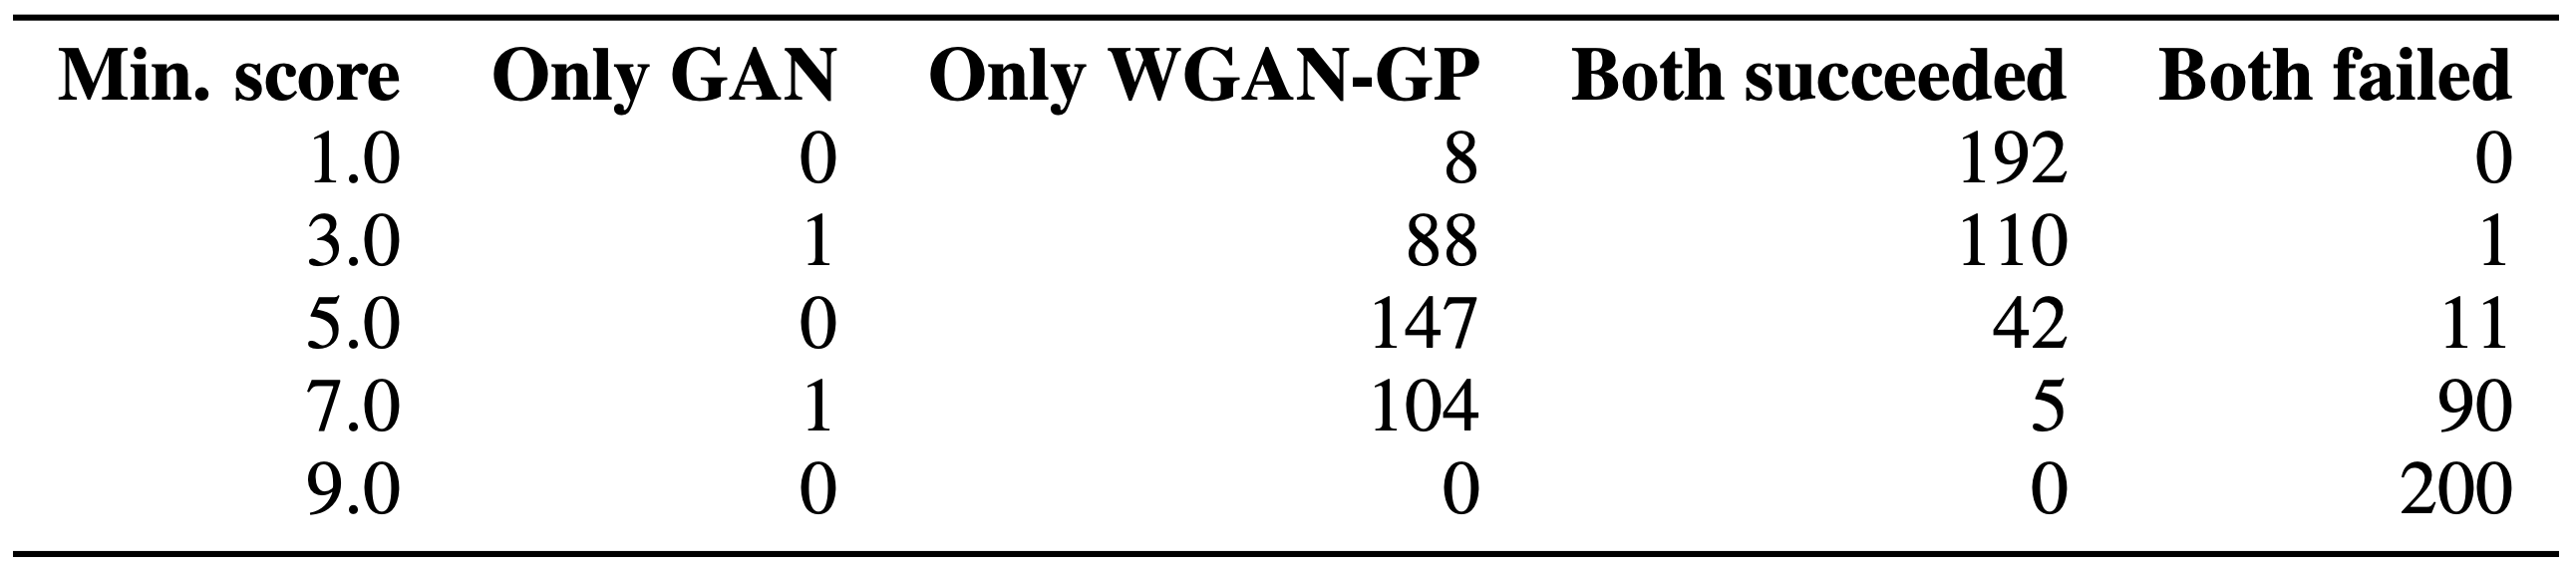
\includegraphics[width=0.65\linewidth]{figs/wgan_gp_wgan}
	\end{figure}
	\vfill
	\hrule\medskip 
	{\scriptsize \href{https://arxiv.org/abs/1704.00028}{https://arxiv.org/abs/1704.00028}}
	
\end{frame}
%=======
\begin{frame}{Wasserstein GAN with Gradient Penalty}
	\begin{figure}
		\centering
		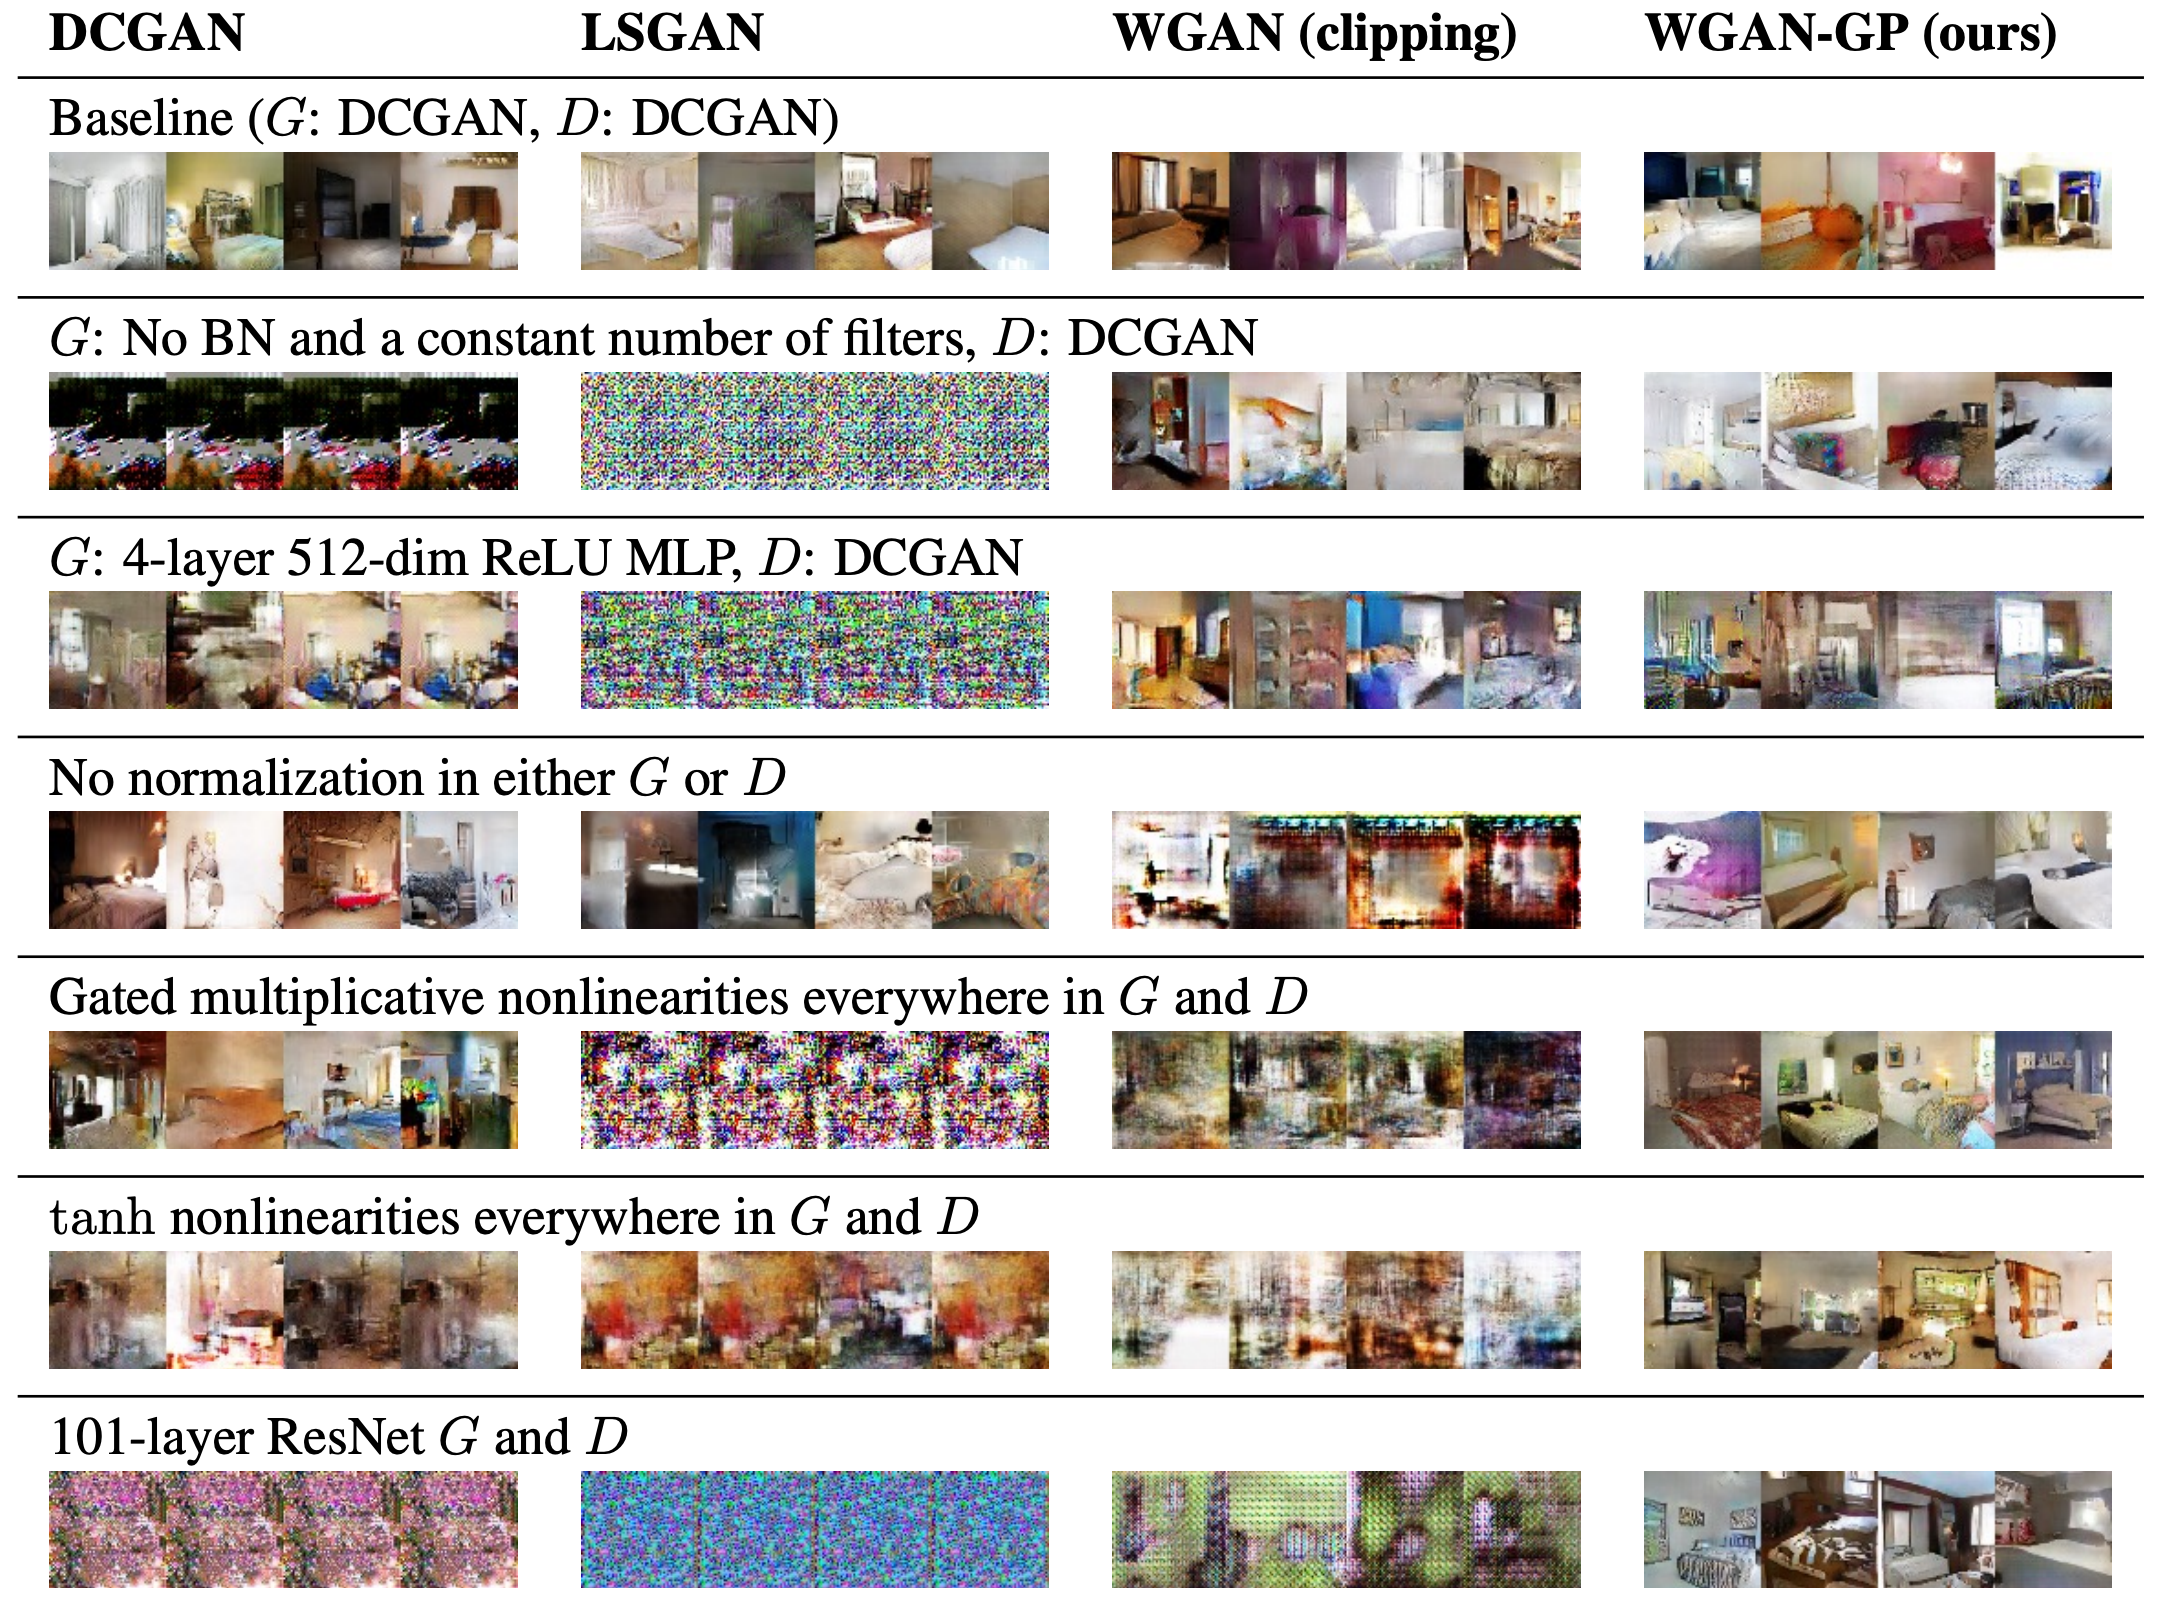
\includegraphics[width=0.95\linewidth]{figs/wgan_gp_results}
	\end{figure}
	\vfill
	\hrule\medskip 
	{\scriptsize \href{https://arxiv.org/abs/1704.00028}{https://arxiv.org/abs/1704.00028}}
	
\end{frame}
%=======
\begin{frame}{Summary}
	\begin{itemize}
		\item Likelihood is not a perfect criteria to measure quality of generative model.
		\item Adversarial learning suggest to solve minimax problem with generator and discriminator.
		\item Vanila GAN tries to optimize (in some sense) Jensen-Shannon divergence.
		\item Mode collapse and vanishing gradients are the two main problems of vanila GAN.
		\item Lots of tips and tricks has to be used to make the GAN training is stable and scalable.
		\item Wasserstein distance is more appropriate objective function for distribution matching problem.
		\item Gradient penalty allows to make Wasserstein GAN even more stable.
	\end{itemize}
\end{frame}
%=======
\begin{frame}{References}
{\tiny
\begin{itemize}
	
	\item \textbf{WGAN}: Wasserstein GAN \\
	\href{https://arxiv.org/abs/1701.07875}{https://arxiv.org/abs/1701.07875} \\
	\textbf{Summary:} Proposed Earth-Mover distance as divergence measure. It shows theoretically that EM distance could be better \\ than KL, JS and TV measures. Kantorovich-Rubinstein duality gives the new objective. All we need to enforce is Lipschitz \\ continuity (e.x. by gradient clipping).
	
	\item \textbf{WGAN-GP}: Improved Training of Wasserstein GANs \\
	\href{https://arxiv.org/abs/1704.00028}{https://arxiv.org/abs/1704.00028} \\
	\textbf{Summary:} Proves that optimal critic has unit gradient almost everywhere. Gradient penalty proposed to enforce Lipchitzness and constraint the critic norm. It greatly improves stability.
\end{itemize}
}
\end{frame}
%=======
\end{document} 